\documentclass[9pt,a5paper,twoside]{extarticle}

\usepackage[inner=13mm,outer=11mm,top=13mm,bottom=15mm,headheight=12pt]{geometry}
\usepackage[T1]{fontenc}
\usepackage[utf8]{inputenc}
\usepackage{tgheros}
\renewcommand{\familydefault}{\sfdefault}
\usepackage[table]{xcolor}
\usepackage{graphicx}
\usepackage{tikz}
\usepackage{tabularx}
\usepackage{booktabs}
\usepackage{enumitem}
\usepackage{microtype}
\usepackage{fancyhdr}
\usepackage{tcolorbox}
\tcbuselibrary{breakable,skins}
\usepackage{hyperref}
\usepackage{xurl}
\graphicspath{{./}{research/workshop-materials/}{../../news/lorentz-center-poster-brief/}{news/lorentz-center-poster-brief/}}

\definecolor{Night}{HTML}{071A2B}
\definecolor{DeepBlue}{HTML}{123B5D}
\definecolor{Sky}{HTML}{3D8EAF}
\definecolor{Aqua}{HTML}{6EC5CB}
\definecolor{Gold}{HTML}{E5AD55}
\definecolor{Mist}{HTML}{EDF5F7}
\definecolor{Cloud}{HTML}{F7FAFB}
\definecolor{Ink}{HTML}{142632}
\definecolor{Muted}{HTML}{526775}
\definecolor{Divider}{HTML}{CAD9DE}
\definecolor{Coral}{HTML}{D9785C}
\definecolor{Violet}{HTML}{7A5BA7}
\definecolor{Teal}{HTML}{2E7D6E}
\definecolor{PaleBlue}{HTML}{92B6D5}
\definecolor{Ochre}{HTML}{B98548}
\definecolor{Slate}{HTML}{65747D}
\definecolor{Magenta}{HTML}{C85A89}

\hypersetup{
  colorlinks=true,
  linkcolor=DeepBlue,
  urlcolor=DeepBlue,
  pdftitle={Workshop Participant Booklet, Version 1.0 — Accelerating Astrophysical Discovery with Foundation Models},
  pdfauthor={Accelerating Astrophysical Discovery consortium},
  pdfsubject={Lorentz Center workshop, 14--18 September 2026},
  pdfkeywords={Version 1.0, 11 August 2026}
}

\color{Ink}
\setlength{\parindent}{0pt}
\setlength{\parskip}{4pt}
\setlist[itemize]{leftmargin=4mm,itemsep=2pt,topsep=2pt}
\setlist[enumerate]{leftmargin=5mm,itemsep=2pt,topsep=2pt}
\emergencystretch=1.5em

\pagestyle{fancy}
\fancyhf{}
\fancyhead[LE]{\scriptsize\color{Muted}ACCELERATING ASTROPHYSICAL DISCOVERY}
\fancyhead[RO]{\scriptsize\color{Muted}PARTICIPANT BOOKLET · SEPTEMBER 2026}
\fancyfoot[C]{\scriptsize\color{Muted}VERSION 1.0 · 11 AUGUST 2026}
\fancyfoot[LE,RO]{\scriptsize\color{Muted}\thepage}
\renewcommand{\headrulewidth}{0pt}
\renewcommand{\footrulewidth}{0pt}

\newcommand{\eyebrow}[1]{%
  {\small\bfseries\color{Sky}\MakeUppercase{#1}}\par\vspace{2mm}}

\newcommand{\pagetitle}[2]{%
  \eyebrow{#1}%
  {\fontsize{20}{22}\selectfont\bfseries\color{Night}#2\par}%
  \vspace{3mm}%
  {\color{Gold}\rule{18mm}{1.4pt}}\par\vspace{4mm}}

\newcommand{\kpanumber}[1]{%
  \tikz[baseline=(char.base)]{%
    \node[circle,fill=DeepBlue,text=white,font=\bfseries\small,inner sep=2.2pt] (char) {#1};}}

\newcommand{\chartdot}[1]{%
  \tikz[baseline=-0.45ex]{\fill[#1] (0,0) circle[radius=1.05mm];}}

\newtcolorbox{infobox}[1][]{
  enhanced,
  colback=Mist,
  colframe=Mist,
  boxrule=0pt,
  borderline west={2.2pt}{0pt}{Sky},
  arc=1.5mm,
  left=3.5mm,right=3.5mm,top=3mm,bottom=3mm,
  #1
}

\newtcolorbox{darkbox}[1][]{
  enhanced,
  colback=Night,
  colframe=Night,
  coltext=white,
  boxrule=0pt,
  arc=1.5mm,
  left=4mm,right=4mm,top=3.5mm,bottom=3.5mm,
  #1
}

\newcommand{\dayheader}[4]{%
  \eyebrow{#1 · #3}%
  {\fontsize{18}{20}\selectfont\bfseries\color{Night}#2\par}%
  \vspace{2.5mm}
  \begin{infobox}
    \textbf{Deliverable}\quad #4
  \end{infobox}
  \vspace{2mm}
}

\newcommand{\slot}[3]{%
  \textbf{#1} & \textbf{#2}\if\relax\detokenize{#3}\relax\else\par\vspace{-1pt}{\scriptsize\color{Muted}#3}\fi\\
  \arrayrulecolor{Divider}\midrule
}

\newenvironment{scheduletable}{%
  \renewcommand{\arraystretch}{1.16}%
  \rowcolors{2}{Cloud}{white}%
  \tabularx{\linewidth}{@{\hspace{1mm}}>{\raggedright\arraybackslash\color{DeepBlue}}p{23mm} >{\raggedright\arraybackslash}X@{\hspace{1mm}}}
  \rowcolor{DeepBlue}\color{white}\bfseries Time & \color{white}\bfseries Session\\
  \arrayrulecolor{DeepBlue}\midrule
}{%
  \endtabularx
}

\begin{document}

% Cover
\thispagestyle{empty}
\hypersetup{pageanchor=false}
\begin{tikzpicture}[remember picture,overlay]
  \fill[Night] (current page.south west) rectangle (current page.north east);
  \node[anchor=north,inner sep=0pt] at (current page.north) {%
    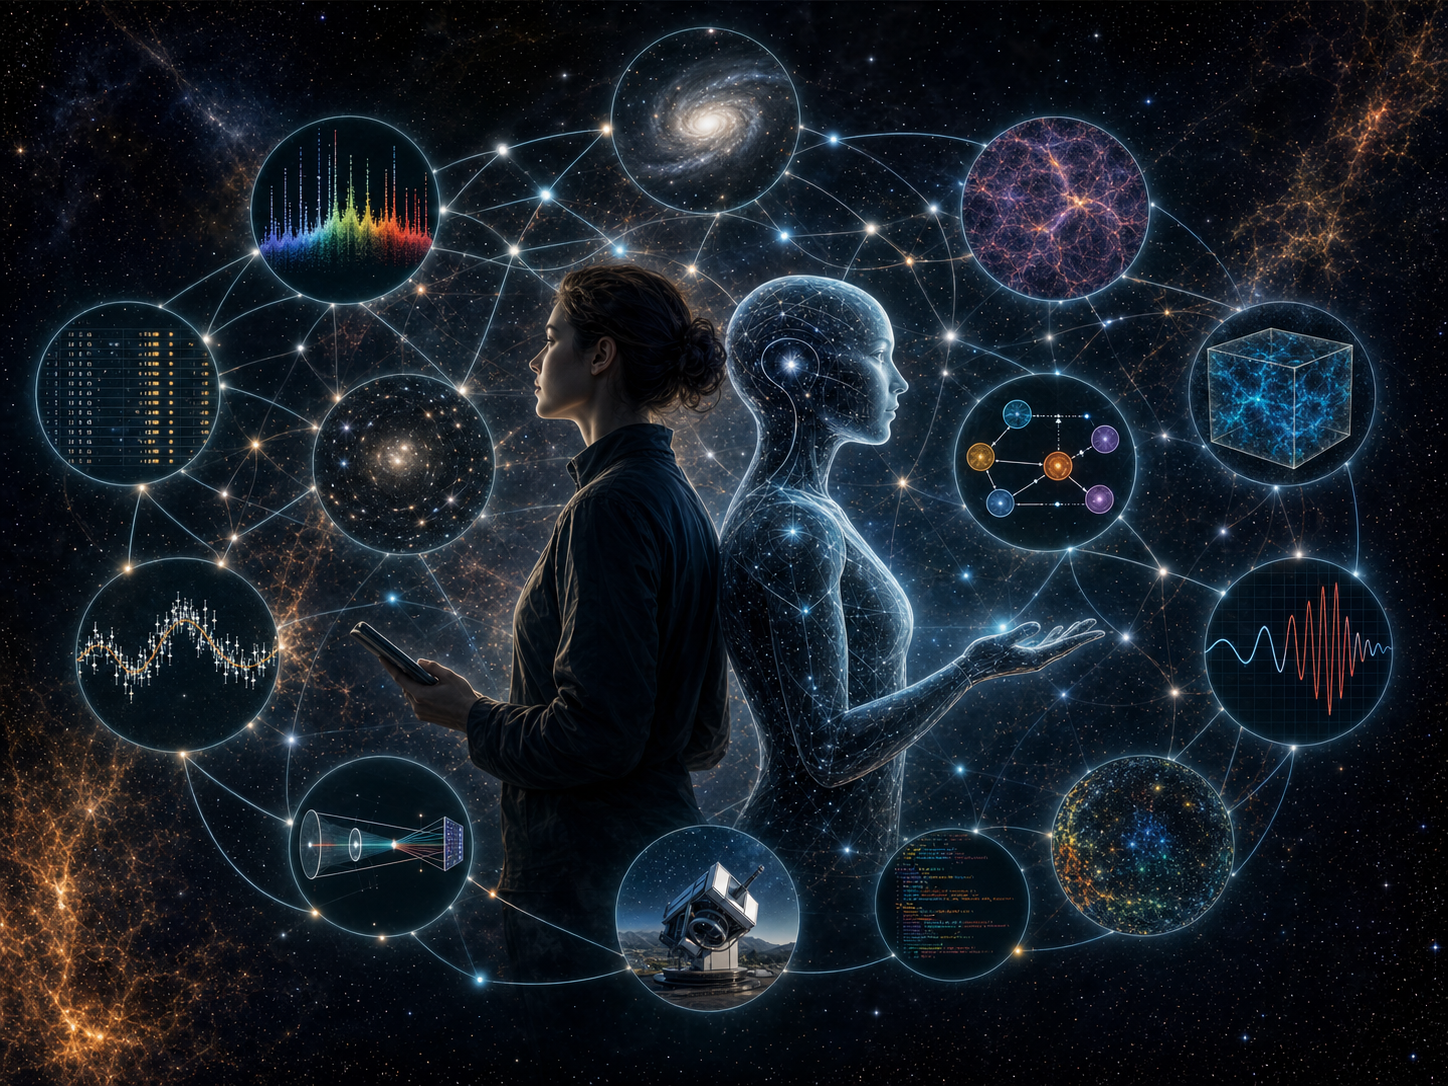
\includegraphics[width=\paperwidth]{joint-human-ai-discovery.png}};
  \fill[shade,left color=Night!95,right color=DeepBlue!92]
    (current page.south west) rectangle ([yshift=-104.8mm]current page.north east);
  \node[anchor=north west,text width=124mm,align=left]
    at ([xshift=12mm,yshift=-112mm]current page.north west) {%
      {\small\bfseries\color{Aqua}LORENTZ CENTER WORKSHOP\par}
      \vspace{4mm}
      {\fontsize{24}{27}\selectfont\bfseries\color{white}
        Accelerating Astrophysical\par Discovery\par}
      \vspace{1mm}
      {\fontsize{15}{18}\selectfont\color{white!86}
        with Foundation Models\par}
      \vspace{5mm}
      {\large\bfseries\color{Gold}Participant booklet\par}
      \vspace{4mm}
      {\small\color{white!86}14--18 September 2026\quad·\quad Leiden, The Netherlands\par}
      \vspace{2.5mm}
      {\scriptsize\bfseries\color{Aqua}VERSION 1.0 · 11 AUGUST 2026\par}
    };
\end{tikzpicture}
\null\newpage

\setcounter{page}{1}
\hypersetup{pageanchor=true}
\pagetitle{Welcome}{A week built for making}

Dear Lorentz Workshop participant,

In a little over a month, we will meet in Leiden for an interactive week devoted to pushing the bounds of how we study the cosmos. We want the workshop to turn diverse expertise into shared decisions, concrete artifacts, and collaborations that continue after Friday.

This booklet introduces the consortium's ambition, explains the initial working set of four Key Problem Areas (KPAs), lays out the working timetable, and suggests a few things to think about before you arrive. You do not need polished proposals. Bring concrete examples, informed questions, and a willingness to build across disciplinary boundaries.

\begin{darkbox}
  {\bfseries\color{Gold}AT A GLANCE}\par\vspace{2mm}
  \begin{tabularx}{\linewidth}{@{}>{\bfseries\color{Aqua}}p{25mm}X@{}}
    Workshop & Accelerating Astrophysical Discovery with Foundation Models\\[2mm]
    Dates & Monday 14 to Friday 18 September 2026\\[2mm]
    Venue & Lorentz Center@omega, Leiden, The Netherlands\\[2mm]
    Start times & Monday at 10:00; Tuesday--Friday at 9:30\\
  \end{tabularx}
\end{darkbox}

\vfill
{\small\color{Muted}The working style is closer to an open-source project hackathon than a sequence of lectures: short framing talks, focused working sessions, plenary synthesis, and a named deliverable each day.}
\newpage

\eyebrow{Workshop community}
{\fontsize{18}{20}\selectfont\bfseries\color{Night}List of participants\par}
\vspace{1.5mm}
{\color{Gold}\rule{18mm}{1.4pt}}\par\vspace{2mm}

{\scriptsize
\setlength{\tabcolsep}{1.2mm}
\renewcommand{\arraystretch}{0.84}
\rowcolors{2}{Cloud}{white}
\begin{tabularx}{\linewidth}{@{\hspace{1mm}}>{\bfseries\color{DeepBlue}}l l >{\raggedright\arraybackslash}X@{\hspace{1mm}}}
  \rowcolor{DeepBlue}\color{white}\bfseries Last name & \color{white}\bfseries First name & \color{white}\bfseries Affiliation\\
  Albert & Joshua G. & California Institute of Technology\\
  Albin & Thomas & Freelancer Scientist\\
  Angeloudi & Eirini & University of Hamburg, Germany\\
  Bester & Hertzog Landman & SARAO, South Africa\\
  Bhihe & Cedric & BSC, Spain\\
  Bulmus & Turan & Google\\
  Callingham & Joseph & ASTRON/UvA\\
  Caron & Sascha & Radboud University\\
  Cheng & Ting-Yun & University of Groningen\\
  Ciuca & Ioana & Stanford University, USA\\
  Cruz & Marcos & Instituto de Física de Cantabria, Spain\\
  Cuesta Lazaro & Carolina & Flatiron Institute / New York University\\
  De la Torre Luque & Pedro & Universidad Autónoma de Madrid (UAM)\\
  Eckner & Christopher & Instituto de Astrofísica de Canarias\\
  Fernández Sopuerta & Carlos & ICE/CSIC, Spain\\
  Glombitza & Jonas & FAU, Germany\\
  Heng & Ik Siong & University of Glasgow, UK\\
  Huertas-Company & Marc & IAC\\
  Huppenkothen & Daniela & University of Amsterdam, The Netherlands\\
  Jain & Divesh & University of Heidelberg\\
  Keenan & Ryan & Max Planck Institute for Astronomy\\
  Keller & Christoph & National Solar Observatory\\
  Khan & Sebastian & Starling Bank\\
  Leonhard & David & University of Bonn\\
  Lopez & Melissa & Nikhef\\
  Loukili & Soulaymane & BSC, Spain\\
  Madireddy & Sandeep & Simons SkAI, Argonne National Laboratory\\
  Pérez Romero & Judit & IFIC (UV/CSIC)\\
  Ruiz de Austri & Roberto & Universidad de Valencia\\
  Samia & Noelle & Simons SkAI\\
  Smirnov & Oleg & Rhodes University \& SARAO\\
  Sotoudeh & Hadi & University of Cambridge\\
  Stevance & Héloïse & Oxford University, UK\\
  Tallada Crespí & Pau & CIEMAT-PIC\\
  Ting & Yuan-Sen & Ohio State University, USA\\
  Vacheret & Antonin & Laboratoire Corpusculaire de Caen UMR 6534, Caen, France\\
  Villaescusa-Navarro & Francisco & Simons Foundation\\
  Weigel & Philip & Harvard University\\
  Zaharijas & Gabrijela & University of Nova Gorica\\
  Zhao & Yue & SURF, NL\\
\end{tabularx}
}

\vspace{3mm}
\begin{tcolorbox}[enhanced,colback=Cloud,colframe=Divider,boxrule=.5pt,arc=1.5mm,left=3.5mm,right=3.5mm,top=2.5mm,bottom=2.5mm]
  {\small\bfseries\color{DeepBlue}Consortium fields}\hfill
  {\scriptsize\color{Muted}Share of field entries}\par\vspace{1.5mm}
  \begin{minipage}[c]{0.34\linewidth}
    \centering
    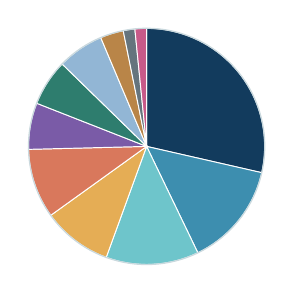
\begin{tikzpicture}
      \path[fill=DeepBlue,draw=white,line width=.35pt] (0,0) -- (90:15mm) arc[start angle=90,end angle=-12.857,radius=15mm] -- cycle;
      \path[fill=Sky,draw=white,line width=.35pt] (0,0) -- (-12.857:15mm) arc[start angle=-12.857,end angle=-64.286,radius=15mm] -- cycle;
      \path[fill=Aqua,draw=white,line width=.35pt] (0,0) -- (-64.286:15mm) arc[start angle=-64.286,end angle=-110,radius=15mm] -- cycle;
      \path[fill=Gold,draw=white,line width=.35pt] (0,0) -- (-110:15mm) arc[start angle=-110,end angle=-144.286,radius=15mm] -- cycle;
      \path[fill=Coral,draw=white,line width=.35pt] (0,0) -- (-144.286:15mm) arc[start angle=-144.286,end angle=-178.571,radius=15mm] -- cycle;
      \path[fill=Violet,draw=white,line width=.35pt] (0,0) -- (-178.571:15mm) arc[start angle=-178.571,end angle=-201.429,radius=15mm] -- cycle;
      \path[fill=Teal,draw=white,line width=.35pt] (0,0) -- (-201.429:15mm) arc[start angle=-201.429,end angle=-224.286,radius=15mm] -- cycle;
      \path[fill=PaleBlue,draw=white,line width=.35pt] (0,0) -- (-224.286:15mm) arc[start angle=-224.286,end angle=-247.143,radius=15mm] -- cycle;
      \path[fill=Ochre,draw=white,line width=.35pt] (0,0) -- (-247.143:15mm) arc[start angle=-247.143,end angle=-258.571,radius=15mm] -- cycle;
      \path[fill=Slate,draw=white,line width=.35pt] (0,0) -- (-258.571:15mm) arc[start angle=-258.571,end angle=-264.286,radius=15mm] -- cycle;
      \path[fill=Magenta,draw=white,line width=.35pt] (0,0) -- (-264.286:15mm) arc[start angle=-264.286,end angle=-270,radius=15mm] -- cycle;
      \draw[Divider,line width=.45pt] (0,0) circle[radius=15mm];
    \end{tikzpicture}
  \end{minipage}\hfill
  \begin{minipage}[c]{0.62\linewidth}
    {\fontsize{6.9}{7.8}\selectfont
    \renewcommand{\arraystretch}{0.96}
    \begin{tabularx}{\linewidth}{@{}c>{\raggedright\arraybackslash}X>{\bfseries\color{DeepBlue}}r@{}}
      \chartdot{DeepBlue} & AI & 28.6\%\\
      \chartdot{Sky} & Cosmology & 14.3\%\\
      \chartdot{Aqua} & Radio & 12.7\%\\
      \chartdot{Gold} & Computational physics & 9.5\%\\
      \chartdot{Coral} & Gravitational waves & 9.5\%\\
      \chartdot{Violet} & Gamma-rays & 6.3\%\\
      \chartdot{Teal} & Neutrinos & 6.3\%\\
      \chartdot{PaleBlue} & Optical & 6.3\%\\
      \chartdot{Ochre} & X-Ray & 3.2\%\\
      \chartdot{Slate} & CRs & 1.6\%\\
      \chartdot{Magenta} & Infrared & 1.6\%\\
    \end{tabularx}}
  \end{minipage}
\end{tcolorbox}
\newpage

\pagetitle{The consortium}{Two connected pillars}

\begin{tcolorbox}[enhanced,colback=DeepBlue,colframe=DeepBlue,coltext=white,boxrule=0pt,arc=2mm,left=5mm,right=5mm,top=5mm,bottom=5mm]
  {\large\bfseries\color{Gold}PILLAR 01}\par\vspace{2mm}
  {\Large\bfseries Design science for human--AI collaboration}\par\vspace{3mm}
  The first goal is to design how future astrophysicists and cosmologists will do science in collaboration with AI. This is more than adding chat interfaces to existing tools. It means redesigning workflows so humans, reasoning language models, simulators, archives, instruments, and foundation models can jointly form hypotheses, retrieve evidence, run checks, update beliefs, and communicate results.
\end{tcolorbox}

\vspace{4mm}

\begin{tcolorbox}[enhanced,colback=Mist,colframe=Mist,boxrule=0pt,arc=2mm,left=5mm,right=5mm,top=5mm,bottom=5mm,borderline west={2.5pt}{0pt}{Gold}]
  {\large\bfseries\color{Sky}PILLAR 02}\par\vspace{2mm}
  {\Large\bfseries\color{Night}Build a joint representation of physical data}\par\vspace{3mm}
  The second goal is to build the technical substrate: a model that learns across observations, simulations, synthetic observations, language, code, and instrumental context. It should support meaningful embeddings for retrieval and serendipity, along with generative capabilities for conditional inference across linked views of the same physical system.
\end{tcolorbox}

\vfill
\begin{infobox}
  \textbf{One shared ambition.} The two pillars meet in an agentic discovery system: reasoning models guide scientific work, the joint-representation model grounds that work in physical evidence, and humans remain responsible for judgement.
\end{infobox}
\newpage

\pagetitle{Key Problem Areas}{KPAs 1 and 2}

The four KPAs are a starting framework, not a fixed list. A central workshop goal is to test whether they frame the right scientific problems---and to refine, combine, replace, or add KPAs as our discussions and use cases demand.

\vspace{2mm}
\begin{tcolorbox}[enhanced,colback=Cloud,colframe=Divider,boxrule=.5pt,arc=1.5mm,left=4mm,right=4mm,top=4mm,bottom=4mm]
  {\large\bfseries\color{Night}\kpanumber{1}\quad Serendipity through embeddings}\par\vspace{2mm}
  A physically meaningful embedding space can surface rare objects, surprising analogues, counterexamples, and neighbouring evidence a scientist may not know to request.

  \textbf{Workshop question}\quad Can it find scientifically meaningful candidates faster and more reliably than current workflows?

  \textbf{Evidence of progress}\quad Positive controls, rare-class retrieval, synthetic anomalies, baseline comparisons, and expert review.
\end{tcolorbox}

\vspace{4mm}
\begin{tcolorbox}[enhanced,colback=Cloud,colframe=Divider,boxrule=.5pt,arc=1.5mm,left=4mm,right=4mm,top=4mm,bottom=4mm]
  {\large\bfseries\color{Night}\kpanumber{2}\quad Generative inference across instruments}\par\vspace{2mm}
  Instruments see the universe through different resolutions, cadences, noise, coverage, and selection effects. Conditional generation may connect those views through super-resolution, deconfusion, gap filling, missing-modality prediction, or cross-instrument reconstruction.

  \textbf{Workshop question}\quad Is the generated view supported by evidence, rather than merely plausible-looking?

  \textbf{Evidence of progress}\quad Controlled degradation, held-out modalities, calibrated uncertainty, forward-model checks, and classical baselines.
\end{tcolorbox}

\vfill
{\small\color{Muted}\textbf{Scientific standard:} useful generative inference must expose what is observed, what is assumed, what remains uncertain, and how the output can be checked.}
\newpage

\pagetitle{Key Problem Areas}{KPAs 3 and 4}

\begin{tcolorbox}[enhanced,colback=Cloud,colframe=Divider,boxrule=.5pt,arc=1.5mm,left=4mm,right=4mm,top=4mm,bottom=4mm]
  {\large\bfseries\color{Night}\kpanumber{3}\quad Observations to physical states}\par\vspace{2mm}
  Multimodal observations could constrain candidate physical states or simulation initial conditions. Candidate states are evolved through system and instrument simulators, then compared back to observations.

  \textbf{Workshop question}\quad Do forward runs remain physically admissible and observationally consistent?

  \textbf{Evidence of progress}\quad Forward-model consistency, stable physical structure, residual analysis, uncertainty, and an auditable chain of assumptions.
\end{tcolorbox}

\vspace{3mm}
\begin{tcolorbox}[enhanced,colback=Cloud,colframe=Divider,boxrule=.5pt,arc=1.5mm,left=4mm,right=4mm,top=4mm,bottom=4mm]
  {\large\bfseries\color{Night}\kpanumber{4}\quad Human--machine discovery}\par\vspace{2mm}
  This is the workflow lens: how should scientists, reasoning language models, tools, simulators, archives, and the joint-representation model form, test, revise, and communicate hypotheses together?

  \textbf{Workshop question}\quad Does the combined workflow improve search, triage, hypothesis generation, validation, or communication without hiding uncertainty or responsibility?
\end{tcolorbox}

\vspace{3mm}
\begin{darkbox}
  \begin{minipage}[t]{0.35\linewidth}
    \vspace{0pt}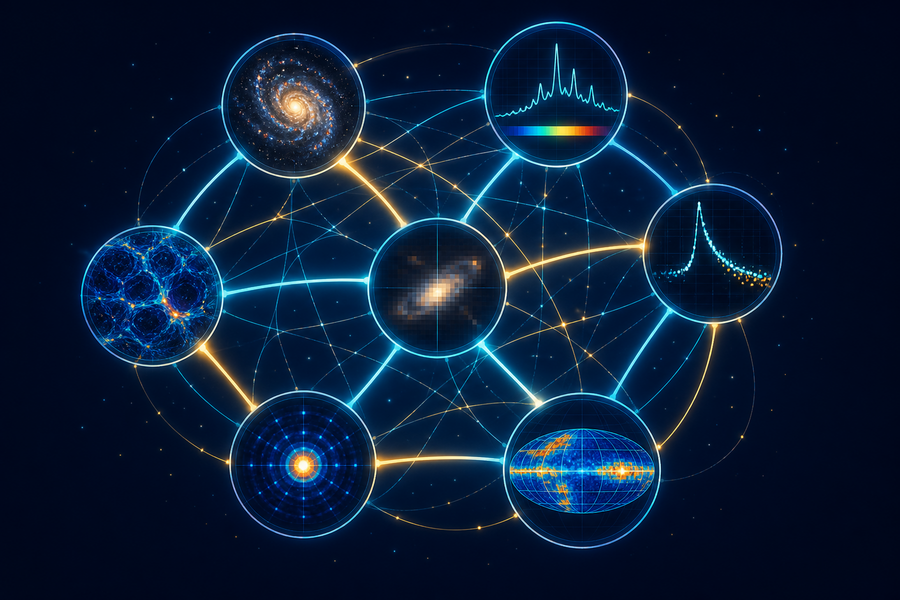
\includegraphics[width=\linewidth]{relevancy-graph.png}\par\vspace{1mm}
    {\fontsize{6.7}{7.7}\selectfont\color{white!65}Nodes are physical data; relevancy links become the training-time attention mask.}
  \end{minipage}\hfill
  \begin{minipage}[t]{0.60\linewidth}
    \vspace{0pt}{\bfseries\color{Gold}THE RELEVANCY GRAPH}\par\vspace{1.5mm}
    We envision a large graph database whose nodes are physical data and whose links encode relevancy. Unlike text, whose sequence yields a causal mask, physical data have no universal order. During self-supervised training, sampled graph connectivity becomes the attention mask. It defines a more general attentional field---cross-modal, many-to-many, and hierarchical---within which the model predicts, reconstructs, or aligns withheld data.
  \end{minipage}
\end{darkbox}
\newpage

\pagetitle{Before Leiden}{Bring ingredients, not finished answers}

\begin{tcolorbox}[enhanced,colback=DeepBlue,colframe=DeepBlue,coltext=white,boxrule=0pt,arc=2mm,left=5mm,right=5mm,top=4.5mm,bottom=4.5mm]
  {\large\bfseries\color{Gold}ASTROPHYSICS + COMPUTATIONAL PHYSICS}\par\vspace{2mm}
  Think about use cases where AI could help humans study the cosmos and do better science if it could understand, reason about, and generate physical data.

  Prepare a list of astrophysical data you can access. Any modality is welcome, including:
  \begin{itemize}[label=\textcolor{Aqua}{\textbullet}]
    \item observations, catalogues, spectra, images, time series, and event lists;
    \item simulation code, snapshots, initial conditions, and synthetic observations;
    \item multimodal observations of the same systems;
    \item instrument responses, calibration context, uncertainties, and provenance.
  \end{itemize}
\end{tcolorbox}

\vspace{4mm}
\begin{tcolorbox}[enhanced,colback=Mist,colframe=Mist,boxrule=0pt,arc=2mm,left=5mm,right=5mm,top=4.5mm,bottom=4.5mm,borderline west={2.5pt}{0pt}{Gold}]
  {\large\bfseries\color{DeepBlue}AI + COMPUTATIONAL INFRASTRUCTURE}\par\vspace{2mm}
  Think about the architectural challenges facing a joint-representation model that must learn deep, self-supervised representations of large physical datasets.

  Also consider the infrastructure required to train across physical datasets that can dwarf the data used to train language models:
  \begin{itemize}[label=\textcolor{Sky}{\textbullet}]
    \item long context, heterogeneous tokenisation, and shared latent spaces;
    \item compute-to-data training across distributed archives and HPC systems;
    \item data access, preprocessing, provenance, monitoring, and validation;
    \item staged scaling, simulator-backed synthetic data, and failure modes.
  \end{itemize}
\end{tcolorbox}

\vfill
{\small\color{Muted}If you span both groups, bring both perspectives. If you span neither exactly, bring the constraints, examples, and questions from your own domain.}
\newpage

\pagetitle{The week}{The week at a glance}

\renewcommand{\arraystretch}{1.22}
\begin{tabularx}{\linewidth}{@{}>{\bfseries\color{DeepBlue}}p{20mm} >{\raggedright\arraybackslash}p{38mm} X@{}}
  \toprule
  Day & Focus & Main deliverable\\
  \midrule
  Monday & Vocabulary, use cases, evaluation & Shared Vocabulary and Discovery-Evaluation Map v0\\
  \addlinespace[1mm]
  Tuesday & Data, representation, provenance & Relevancy Graph v0 for selected use cases\\
  \addlinespace[1mm]
  Wednesday & Architecture and training & Architecture and Training Protocol v0\\
  \addlinespace[1mm]
  Thursday & MVP and hackathon & MVP Implementation Plan and Hackathon Artifacts v0\\
  \addlinespace[1mm]
  Friday & Roadmap, governance, funding & Consortium Roadmap and Funding Package v0\\
  \bottomrule
\end{tabularx}

\vspace{5mm}
\begin{darkbox}
  {\bfseries\color{Gold}THE HAND-OFF}\par\vspace{2mm}
  Monday chooses what matters. Tuesday defines the relationships the data and system must respect. Wednesday turns those constraints into a model and training path. Thursday turns that design into workstreams and artifacts. Friday gives the work owners, resources, governance, and continuity.
\end{darkbox}

\vspace{4mm}
\begin{infobox}
  \textbf{Working rhythm}\quad Each day combines brief framing, active work, plenary synthesis, and a concrete closeout. Tuesday--Thursday begin by reviewing overnight AI work; Monday--Wednesday end by agreeing what the AI should prepare for the next morning. Coffee breaks and lunches are part of the programme: use them to connect ideas across disciplines.
\end{infobox}

\vfill
{\small\color{Muted}Formal working hours are 10:00--16:30 on Monday, 9:30--17:00 Tuesday--Thursday, and 9:30--13:30 on Friday. The building is open for arrivals and coffee from 09:00 on Monday.}
\newpage

\dayheader{Monday}{Use cases and discovery workflows}{10:00--16:30}{Shared Vocabulary and Discovery-Evaluation Map v0}

\begin{scheduletable}
  \slot{09:00--10:00}{Arrival and coffee}{The formal programme begins at 10:00.}
  \slot{10:00--10:30}{Kickoff talk}{AI-first science, the two pillars, and KPAs as a starting framework.}
  \slot{10:30--12:00}{Science 2.0 + use cases}{Work from long-term visions back to concrete workflows and candidate use cases.}
  \slot{12:00--13:30}{Lunch}{}
  \slot{13:30--14:30}{Plenary synthesis}{Share, refine, and select a small set of flagship use cases.}
  \slot{14:30--15:00}{Coffee break}{}
  \slot{15:00--16:15}{Define evaluation targets}{Controls, baselines, anomaly tests, forward checks, uncertainty, provenance, and human review.}
  \slot{16:15--16:30}{Closeout + AI brief}{Confirm cases, evaluations, owners, and the overnight synthesis for Tuesday.}
  \slot{16:30 onward}{Welcome reception}{Informal continuation after the formal programme.}
\end{scheduletable}

\vfill
\begin{infobox}
  \textbf{Keep asking}\quad What would count as evidence that this workflow produces better science, rather than simply more output?
\end{infobox}
\newpage

\dayheader{Tuesday}{Data, representation, and provenance}{9:30--17:00}{Relevancy Graph v0 for Monday's selected use cases}

\begin{scheduletable}
  \slot{9:30--10:00}{Kickoff + overnight review}{Correct Monday's synthesis; introduce the graph and tokenisation challenges.}
  \slot{10:00--10:30}{Map data objects}{Use participants' lists to connect cases to observations, simulations, instruments, code, and provenance.}
  \slot{10:30--11:00}{Coffee break}{}
  \slot{11:00--12:00}{Graph working session}{Define nodes, relevancy links, metadata, provenance, ambiguities, and training relationships.}
  \slot{12:00--13:30}{Lunch}{}
  \slot{13:30--14:30}{Plenary graph synthesis}{Share group results and assemble Relevancy Graph v0.}
  \slot{14:30--15:00}{Coffee break}{}
  \slot{15:00--16:30}{Tokenisation + constraints}{Record what representations must preserve and the constraints for Wednesday.}
  \slot{16:30--17:00}{Closeout + AI brief}{Confirm owners; commission a draft schema or prototype and architecture primer.}
\end{scheduletable}

\vfill
\begin{infobox}
  \textbf{Keep asking}\quad What relationship makes these objects scientifically relevant to one another, and what provenance must survive every transformation?
\end{infobox}
\newpage

\dayheader{Wednesday}{Long-context architecture and training}{9:30--17:00}{Architecture and Training Protocol v0}

\begin{scheduletable}
  \slot{9:30--10:00}{Kickoff + overnight review}{Review the primer and graph work; frame long-context, recurrent-depth, and graph-attention challenges.}
  \slot{10:00--10:30}{Translate graph constraints}{Preserve typed objects, relationships, units, uncertainty, and metadata.}
  \slot{10:30--11:00}{Coffee break}{}
  \slot{11:00--12:00}{Architecture working session}{Use AI to sketch candidate architecture families, objectives, and training hypotheses.}
  \slot{12:00--13:30}{Lunch}{}
  \slot{13:30--14:30}{Plenary synthesis}{Compare designs, identify common components, and retain justified alternatives.}
  \slot{14:30--15:00}{Coffee break}{}
  \slot{15:00--16:30}{Training + prototype brief}{Set objectives, simulator feedback, deployment, validation, scaling, risks, and Thursday artifacts.}
  \slot{16:30--17:00}{Closeout + AI brief}{Confirm hypotheses, protocol, owners, and overnight prototype work.}
  \slot{17:00--20:00}{Workshop dinner}{Informal continuation after the formal programme.}
\end{scheduletable}
\newpage

\dayheader{Thursday}{MVP architecture and hackathon}{9:30--17:00}{MVP Implementation Plan and Hackathon Artifacts v0}

\begin{scheduletable}
  \slot{9:30--10:00}{Kickoff + overnight review}{Review the prototype, state the MVP target, and share AI-assisted coding approaches.}
  \slot{10:00--10:30}{Self-organise workstreams}{Choose concrete artifacts and owners across technical, documentation, and roadmap work.}
  \slot{10:30--11:00}{Coffee break}{}
  \slot{11:00--12:00}{Open hackathon I}{Build toy-scale artifacts in the main room or breakouts.}
  \slot{12:00--13:30}{Lunch}{}
  \slot{13:30--14:30}{Open hackathon II}{Continue building; demonstrate useful progress as it appears.}
  \slot{14:30--15:00}{Coffee break}{}
  \slot{15:00--16:15}{Show-and-tell + integration}{Demonstrate artifacts, connect them to use cases and evaluation, and identify gaps.}
  \slot{16:15--17:00}{Closeout + Friday handoff}{Confirm artifacts, issues, owners, next work, and Friday's resource questions.}
\end{scheduletable}

\vfill
{\small\color{Muted}\textbf{Thursday rule:} every artifact should connect to a use case, a model capability, and an evaluation target.}
\newpage

\dayheader{Friday}{Roadmap, governance, and funding}{9:30--13:30}{Consortium Roadmap and Funding Package v0}

\begin{scheduletable}
  \slot{9:30--10:00}{Funding + continuity kickoff}{Review the week's artifacts and frame resources, partnerships, deployment, and maintenance.}
  \slot{10:00--10:30}{Map resource needs}{Compute, data, simulators, archives, expertise, funding, and missing roles.}
  \slot{10:30--11:00}{Coffee break}{}
  \slot{11:00--11:30}{Funding and partnerships}{Identify opportunities, partners, institutional support, and lead owners.}
  \slot{11:30--12:00}{Commitments + roadmap}{Record desired participation; confirm milestones, owners, cadence, and invitees.}
  \slot{12:00--13:30}{Closing lunch}{Final confirmations and departures.}
\end{scheduletable}

\vspace{4mm}
\begin{darkbox}
  {\bfseries\color{Gold}PRACTICAL MATTERS}\par\vspace{2mm}
  Discounted hotel reservations are limited, so please book as soon as possible if you need accommodation.

  For practical questions or help with accommodation, contact Maria Krebbers at
  \href{mailto:acceleratingastrophysical@lorentzcenter.nl}{acceleratingastrophysical@lorentzcenter.nl}.
\end{darkbox}

\vfill
\begin{center}
  {\small\bfseries\color{DeepBlue}accelerating-astrophysical-discovery.github.io}\par
  \vspace{2mm}
  {\scriptsize\color{Muted}Bring a use case. Bring a constraint. Leave with something we can build together.}
\end{center}

\end{document}
